\documentclass{beamer}

\usepackage{graphicx}
\usepackage{listings}
\usepackage{color}
\usepackage{hyperref}

\usetheme{Madrid}
\usecolortheme{beaver}


\title{Numerical Approximation of Non-Linear Equations Using Adams-Bashforth Method}
\author[Makau, Opiyo, Luseno] 
{A.~M.~Makau\inst{1} \and S.~Opiyo\inst{2} \and M.~Luseno\inst{3}}

\institute[JKUAT]
{
  \inst{1}%
  SCT211-0469/2021
  
  \and
  \inst{2}%
  SCT211-0509/2021

  \and
  \inst{3}%
  SCT211-0588/2021
}

\date{March 28, 2023}

\begin{document}

\begin{frame}
  \titlepage
\end{frame}

\begin{frame}{Introduction}

\begin{itemize}
    \item Non-linear equations are difficult to solve analytically.
    \item Numerical methods are often used to approximate the solutions.
    \item One such method is the Adams-Bashforth method.
    \item The Adams-Bashforth method is a predictor-corrector method that uses past values of the function to approximate future values.
    \item The predictor step uses previous function evaluations to predict the next value.
    \item The corrector step uses a weighted average of function evaluations to correct the prediction.
    \item Let's consider an example to illustrate the method.
\end{itemize}

\end{frame}

\begin{frame}{Adams-Bashforth Method: Example}
    
Consider the initial value problem
\begin{align*}
y'(t) &= -2ty(t)^2, \\
y(0) &= 1,
\end{align*}
with solution $y(t) = \frac{1}{1+t^2}$. \\ Suppose we want to approximate $y$ at $t=1$ using the Adams-Bashforth method.

\end{frame}

\begin{frame}{Adams-Bashforth Method: Example (cont'd)}

\begin{itemize}
    \item We start by computing the values of $y$ and $t$ for $t=0$ and $t=0.5$, using the fourth-order Runge-Kutta method or any other method.
    \item Let $w_0=y(0)$ and $w_1=y(0.5)$ be the initial values.
    \item The Adams-Bashforth method is a predictor-corrector method that uses the formula
    $$w_{i+1} = w_i + \frac{h}{2}\left(3f(t_i,w_i)-f(t_{i-1},w_{i-1})\right), \quad i=1,2,\ldots,$$
    to compute the next approximations.
\end{itemize}

\end{frame}

\begin{frame}{Adams-Bashforth Method: Example (cont'd)}
    
Using $h=0.5$, we have

\begin{itemize}
    \item $w_0=1$, $w_1=0.8$ (using fourth-order Runge-Kutta)
    \item $w_2 = w_1 + \frac{h}{2}\left(3f(t_1,w_1)-f(t_0,w_0)\right)$
    \item $w_2 = 0.6396$
    \item The exact solution is $y(1)=\frac{1}{2}$.
    \item The error is $|w_2 - y(1)| \approx 0.1396$.
\end{itemize}

\end{frame}

\begin{frame}{Non-Linear Population Equation}
  \begin{itemize}
    \item A non-linear population equation is given by:
      $$\frac{dy}{dt} = 0.2y - 0.01y^2$$
    \item This equation describes how a population $y$ changes over time $t$.
    \item The equation is non-linear due to the quadratic term $y^2$.
  \end{itemize}
\end{frame}

\begin{frame}{Numerical Approximation}
  \begin{itemize}
    \item We will use the Adams-Bashforth method to approximate the solution to the non-linear population equation.
    \item This method is a multi-step method that uses a predictor-corrector scheme.
    \item The Taylor method is used to compute the first step.
  \end{itemize}
\end{frame}

\begin{frame}[fragile]{Python Code (Part 1)}
  \begin{lstlisting}[language=Python,basicstyle=\ttfamily,breaklines=true,keywordstyle=\color{blue}]
  # Python code for numerical approximation
  import numpy as np
  import matplotlib.pyplot as plt
  import pandas as pd
  
  # Define the function f(y, t)
  def f(y, t):
      return 0.2 * y - 0.01 * y**2
  
  # Set the initial conditions
  y0 = 6
  t0 = 2000
  tf = 2020
  h = 1
  \end{lstlisting}
\end{frame}

\begin{frame}[fragile]{Python Code (Part 2)}
  \begin{lstlisting}[language=Python,basicstyle=\ttfamily,breaklines=true,keywordstyle=\color{blue}]
  # Compute the number of steps
  N = int((tf - t0) / h)
  
  # Create arrays to store the solution
  t = np.zeros(N+1)
  y = np.zeros(N+1)
  t[0] = t0
  y[0] = y0
  
  # Use the Taylor method to compute the first step
  y[1] = y[0] + h * f(y[0], t[0]) + h**2 / 2 * (f(y[0], t[0]) - 0.2 * y[0])
  t[1] = t[0] + h
  
  \end{lstlisting}
\end{frame}

\begin{frame}[fragile]{Python Code (Part 3)}
  \begin{lstlisting}[language=Python,basicstyle=\ttfamily,breaklines=true,keywordstyle=\color{blue}]
  # Use the Adams-Bashforth method to compute the remaining steps
for i in range(2, N+1):
  # Predictor step
  y_pred = y[i-1] + h * (3/2 * f(y[i-1], t[i-1]) - 1/2 * f(y[i-2], t[i-2]))
  t_pred = t[i-1] + h
  
  # Corrector step
  y[i] = y[i-1] + h * (5/12 * f(y_pred, t_pred) + 2/3 * f(y[i-1], t[i-1]) - 1/12 * f(y[i-2], t[i-2]))
  t[i] = t[i-1] + h
  
  \end{lstlisting}
\end{frame}

\begin{frame}[fragile]{Python Code (Part 4)}
  \begin{lstlisting}[language=Python,basicstyle=\ttfamily,breaklines=true,keywordstyle=\color{blue}]
  
  # Create a table of the numerical approximation
  data = {'time t_i': t, 'Adams approx of non-linear y': y}
  df = pd.DataFrame(data)
  print(df)
  
  # Plot the solution
  plt.plot(t, y, label='Adams-Bashforth Method')
  plt.title('Non Linear Population Equation')
  plt.legend(loc='best')
  plt.xlabel('time (yrs)')
  plt.ylabel('Population in billions')
  plt.show()
  \end{lstlisting}
\end{frame}


\begin{frame}{Results}
  \begin{itemize}
    \item The numerical approximation of the non-linear population equation is stored in arrays \texttt{t} and \texttt{y}.
    \item A table of the numerical approximation is created using the \texttt{pandas} library.
    \item A plot of the solution is created using the \texttt{matplotlib} library.
  \end{itemize}
\end{frame}

\begin{frame}{Table of Numerical Approximation}
    \centering
        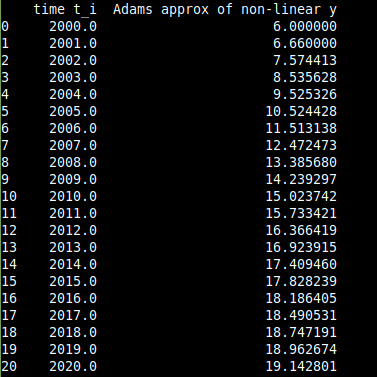
\includegraphics[width = 8cm] {table}
\end{frame}

\begin{frame}{Plot of The Solution}
    \centering
        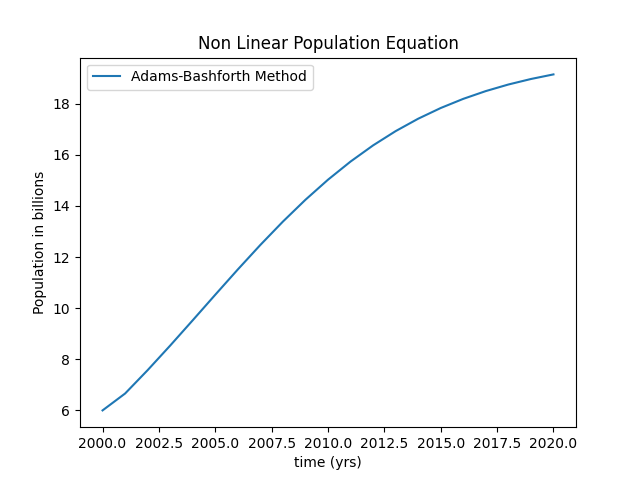
\includegraphics[width = 10cm]{plot}
    \end{frame}

\end{document}
